\documentclass[11pt]{article}
\usepackage[margin=1in]{geometry}
\usepackage{amsmath,amssymb,amsthm,booktabs,array}
\usepackage{graphicx}
\usepackage[T1]{fontenc}
\usepackage[utf8]{inputenc}
\usepackage{lmodern}
\usepackage[hyphens]{url}
\usepackage[colorlinks=true,linkcolor=blue,citecolor=blue,urlcolor=blue]{hyperref}
\newtheorem{theorem}{Theorem}[section]
\newtheorem{corollary}[theorem]{Corollary}
\newtheorem{lemma}[theorem]{Lemma}
\newtheorem{proposition}[theorem]{Proposition}
\newcommand{\C}{\mathbb C}
\newcommand{\R}{\mathbb R}
\newcommand{\NC}{\operatorname{NC}}
\newcommand{\Fix}{\operatorname{Fix}}
\newcommand{\rank}{\operatorname{rank}}
\newcommand{\Park}{\operatorname{Park}}
\newcommand{\Cl}{\operatorname{Cl}}
\setlength{\emergencystretch}{2em}
\raggedbottom
\pagestyle{plain}
\title{The weak parking-space conjecture}
\author{P. Graham\\ \small\url{https://orcid.org/0009-0007-8493-1505}}
\date{October 23, 2026}
\hypersetup{pdfauthor={P. Graham},pdftitle={The weak parking-space conjecture}}
\begin{document}
\maketitle
\begingroup
\renewcommand{\thefootnote}{}
\footnotetext{The proofs, the computation programs, the certificate checkers and the text were produced by AI models (from OpenAI and Anthropic), working under the author's direction.}
\endgroup
\begin{abstract}
Armstrong, Reiner and Rhoades conjectured in 2012 that the noncrossing
and algebraic parking spaces of an irreducible finite real reflection
group have the same character under the reflection group and Coxeter
rotation. We prove their weak conjecture in types $E_7$ and $E_8$, its
last two open real types, completing the conjecture. The proof expresses
fixed parking functions as intersections of conjugacy classes with
cosets of pointwise parabolic subgroups. Complete finite certificates
verify these intersections and the noncrossing interval, using exact
arithmetic. Together with the previously established types, the result
gives the conjectured complex representation isomorphism for every
irreducible finite real reflection group. The assertion concerns the
original parking spaces, with Fuss parameter $1$.
\end{abstract}

\section{Introduction}
We complete the weak form of the parking-space conjecture of Drew
Armstrong, Victor Reiner and Brendon Rhoades, first posted on
April 8, 2012~\cite{ARR}. Let $W$ be an irreducible finite real
reflection group on a real vector space $V$, let $c$ be a Coxeter
element, let $h$ be its order, and put $C=\langle c\rangle$ and
$\omega=\exp(2\pi i/h)$. A noncrossing flat is the fixed space of an
element of the absolute-order interval $[1,c]$; this interval is defined
in Section~\ref{sec:definitions}. For a flat $X$, let $P_X$ be its
pointwise stabilizer in $W$. The noncrossing parking set is
\[
 \Park^{\NC}_W=\{[x,X]: X\text{ is a noncrossing flat},\ xP_X\in W/P_X\},
\]
where $[x,X]$ records the coset $xP_X$ as well as $X$. Its action is
$(w,c^d)[x,X]=[wxc^{-d},c^dX]$.

\begin{theorem}\label{thm:main}
For $W$ of type $E_7$ or $E_8$, every $w\in W$ and every integer $d$
satisfy
\begin{equation}\label{eq:main}
 \bigl|\Fix_{\Park^{\NC}_W}(w,c^d)\bigr|
       =(h+1)^{\dim_{\C}\ker(w-\omega^d I\mid V\otimes_{\R}\C)}.
\end{equation}
Here $h=18$ in type $E_7$ and $h=30$ in type $E_8$.
\end{theorem}

The contribution is the two exceptional-type character computations
requested in Armstrong--Reiner--Rhoades~\cite[Problem~11.1]{ARR}.
Their character formula and reduction to these remaining types are
reused. The main computational difficulty is counting fixed cosets with
Coxeter rotation still present: counting only the $W$-action omits the
condition for nontrivial $c^d$. The reduction below retains every cyclic
exponent, and compresses the count using cyclic orbits of flats and
conjugacy classes of their parabolic normalizing subgroups. A separate
exhaustive downward-closure check establishes that no noncrossing flat
is omitted.

To identify the exact conjecture, let $\Park^{\mathrm{alg}}_W$ denote
the algebraic parking space of~\cite[Section~2.5]{ARR}, described in
Section~\ref{sec:definitions}. With the hypotheses on $W$ and $C$
above, the concluding sentence of their weak Main Conjecture is:
\begin{quote}
``Then one has an isomorphism of $W\times C$-representations''
\[
 \C[\Park^{\mathrm{alg}}_W]
       \cong_{\C[W\times C]}\C[\Park^{\NC}_W].
\]
\end{quote}
This is equation~(2.7) of~\cite[Section~2.6]{ARR}; the statement already
appears in the first public version. The bracket notation in this
quotation is retained from that source.

\begin{corollary}\label{cor:all}
The weak Main Conjecture of Armstrong, Reiner and Rhoades holds for
every irreducible finite real reflection group: its algebraic and
noncrossing parking spaces are isomorphic as complex
$W\times C$-representations.
\end{corollary}

Table~\ref{tab:prior} gives the published results used for the other
types, with the precise locations in~\cite{ARR}. Christian Stump's
software established the earlier exceptional-type computations, as
credited immediately after that paper's Table~1. Brendon Rhoades
subsequently proved the intermediate conjecture in type $A$ for every
Fuss parameter and related it to the generic strong form
\cite[Theorems~1.1--1.2 and Table~1]{Rhoades}. His earlier
\emph{Parking structures: Fuss analogs}~\cite{RhoadesFuss} developed
the Fuss generalization. Those stronger and more general results are
not needed for the original parameter considered here.

\begin{table}[ht]
\centering
\caption{The prior-type bridge for Corollary~\ref{cor:all}. Strong and
intermediate forms each imply the weak form. All references in the
last column are to~\cite{ARR}.}
\label{tab:prior}
\begin{tabular}{lll}
\toprule
Types & Previously established form & Location\\
\midrule
$A_1$, $I_2(m)$ & Strong & Corollary~2.14\\
$A_r$ & Weak & Section~8, equation~(8.1)\\
$B_r/C_r$ & Intermediate & Section~6.2\\
$D_r$ & Intermediate & Section~7.2\\
$H_3,H_4,F_4,E_6$ & Weak, by computation & Table~1 and following paragraph\\
\bottomrule
\end{tabular}
\end{table}

Several nearby results distinguish why the cyclic factor matters.
Theo Douvropoulos and Matthieu Josuat-Verg\`es established the
noncrossing parking character for the $W$-action in all real types,
including $E_7$ and $E_8$, for arbitrary Fuss parameter
\cite[Section~3.2, Theorem~3.10]{DJV}; the discussion in that section
explicitly separates the cyclic enhancement. Yosuke Ito and Soichi
Okada classify when generalized parking class functions are
$W$-characters or permutation characters
\cite[Theorem~1.4 and Section~7.2]{IO}. These existence statements do
not identify the prescribed noncrossing $W\times C$-action. Jason
Stack extends the parking-space construction to well-generated complex
reflection groups, with $G_{34}$, $E_7$ and $E_8$ expressly excluded
from the hypotheses of his main results
\cite[Theorems~1.3 and 3.19]{Stack}. Jason Stack and Nathan Williams
study homogeneous systems of parameters and the resulting graded and
ungraded $W$-modules~\cite[Section~1.2]{SW}; their credit to
Douvropoulos--Josuat-Verg\`es for the $E_7,E_8$ noncrossing character
concerns the $W$-action. Theorem~\ref{thm:main} supplies the full cyclic
character comparison in these two real types.

The conclusion is equality of complex characters and hence a
representation isomorphism. It does not supply an equivariant bijection
of the underlying sets, prove the intermediate or strong conjecture,
treat arbitrary Fuss parameter, or address $G_{34}$. The proof is
computer-assisted and has not yet been reviewed by experts.

Section~\ref{sec:overview} gives the proof strategy.
Section~\ref{sec:definitions} fixes the reflection and parking-space
definitions. Section~\ref{sec:reduction} derives the finite counting
formula and proves the interval-cover criterion.
Section~\ref{sec:computation} describes the certificates, the exact
comparisons and the trusted computational boundary.

\section{Proof overview}\label{sec:overview}
The proof reduces the large parking sets to small group-theoretic
counts. The algebraic side is already known: Armstrong--Reiner--Rhoades
give its value as the right side of~\eqref{eq:main}
\cite[Proposition~2.15]{ARR}. It therefore suffices to compute every
value of the noncrossing parking character.

Fix a noncrossing flat $X$. A parking point over $X$ can be fixed by
$(w,c^d)$ only if $c^dX=X$. In that case its coset condition becomes
$x^{-1}wx\in P_Xc^d$. Consequently the contribution over $X$ is a
centralizer factor times the size of the intersection of a $W$-conjugacy
class with $P_Xc^d$. Flats in the same $C$-orbit make equal
contributions. If this orbit has length $\ell$, the group
$K=\langle P_X,c^\ell\rangle$ contains $P_X$ as a normal subgroup with
cyclic quotient. The coset $P_Xc^d$, when relevant, is a union of
$K$-conjugacy classes. Thus complete class lists for $W$ and these
groups $K$ suffice to compute the entire character.

There are two completeness obligations. First, the list of
noncrossing elements must be the whole absolute-order interval, not
just a collection with the expected cardinality. Starting from $c$,
closure under every reflection step that lowers reflection length
proves this by a reduced-factorization argument. Second, the supplied
class representatives must cover $W$ and each $K$. Centralizer-derived
class sizes, pairwise nonconjugacy, and their sum establish these
covers. Conjugating witnesses then determine how the $K$-classes lie in
$W$-classes, without relying on class labels.

Two implementations check these certificates and recompute all
character values. Both use the same exact GAP group kernel. The
mathematical reduction and that common computational trust are stated
explicitly below.

\section{Reflection and parking spaces}\label{sec:definitions}
This section relates the finite objects counted in the proof to the
parking spaces in the conjecture.

As a small example, in type $A_1$ the group is $W=\{1,s\}$ acting on
a line, and $c=s$. There are two noncrossing flats, the whole line
$V$ and $\{0\}$. Their pointwise stabilizers are $\{1\}$ and $W$,
respectively, so the parking set has two points over $V$ and one over
$\{0\}$. The element $(1,s)$ fixes only the point over $\{0\}$;
the element $(s,s)$ fixes all three. These are the values $3^0$ and
$3^1$ in~\eqref{eq:main}.

In type $A_2$, the group is the symmetry group of an equilateral
triangle. Its five noncrossing flats are the plane, the three reflection
lines, and the origin. Figure~\ref{fig:a2} shows these flats, their
Coxeter rotation, and the sizes of their coset fibers. The parking
points are the cosets over each flat, rather than points drawn on a line.

\begin{figure}[ht]
\centering
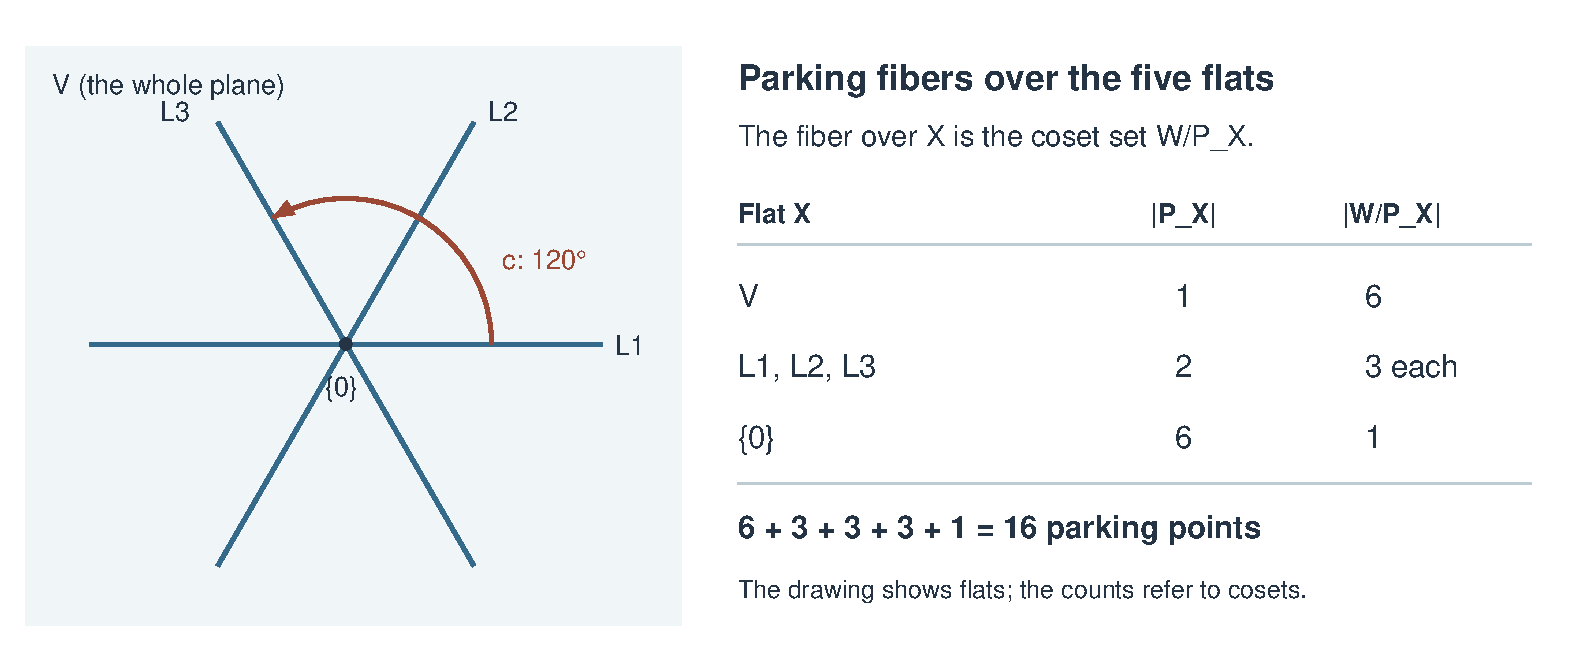
\includegraphics[width=\textwidth]{../data/a2.pdf}
\caption{The type-$A_2$ parking construction. Coxeter rotation permutes
the three lines. The fiber over a flat $X$ is $W/P_X$; its size is
shown on the right. This small example illustrates the definition;
the exceptional-type proof uses the separate certificates below.}
\label{fig:a2}
\end{figure}

Let $T$ be the set of reflections of $W$. The reflection length
$\ell_T(g)$ is the least number of factors in an expression of $g$ as
a product of elements of $T$. Absolute order is defined by
\[
 u\leq_T v\quad\Longleftrightarrow\quad
 \ell_T(v)=\ell_T(u)+\ell_T(u^{-1}v),
 \qquad \NC(W,c)=[1,c]_T.
\]
Carter's formula gives $\ell_T(g)=\rank(I-g)$ in the real reflection
representation~\cite[Section~2]{Carter}; see also
\cite[Section~2.1]{ARR}. The map $u\mapsto\Fix_V(u)$ is injective on
$\NC(W,c)$ by the noncrossing-flat embedding of Brady and Watt
\cite[Theorem~2]{BW}, used in~\cite[Definition~2.2]{ARR}. Its image
is the set of noncrossing flats. With $P_X$ the pointwise stabilizer,
the parking set and action in the introduction agree with
\cite[Definition~2.6 and Section~2.3]{ARR}.

Write $n=\dim_{\R}V$. For the algebraic space, choose coordinates
$x_1,\ldots,x_n$ on the
complexified reflection representation and a homogeneous system of
parameters $\Theta=(\theta_1,\ldots,\theta_n)$ of degree $h+1$ for which
the linear map $x_i\mapsto\theta_i$ from the dual reflection
representation is $W$-equivariant. Here a homogeneous
system of parameters means homogeneous polynomials for which the
quotient by their ideal is finite-dimensional. The algebraic parking
module is
\[
 \C[V\otimes_{\R}\C]/(\theta_1-x_1,\ldots,\theta_n-x_n),
\]
with the $W$-action on polynomials induced by its action on $V$, and
with $c$ acting on a homogeneous polynomial of degree $j$ by
$\omega^{-j}$; see~\cite[Section~2.5, equation~(2.4) and Definition~2.10]{ARR}. Their
Propositions~2.11 and~2.15 show that its character is independent of
the permitted choice of $\Theta$ and equals
$(h+1)^{\dim_{\C}\ker(w-\omega^dI)}$ at $(w,c^d)$. This is the
only algebraic input needed in the comparison.

The finite model in type $E_n$, for $n=7,8$, uses the simple-root
Gram matrix $A$ with diagonal entries $2$ and off-diagonal entry $-1$
on the edges
\[
 (1,3),\ (3,4),\ (2,4),\ (4,5),\ldots,(n-1,n),
\]
and zero elsewhere. Let $e_i$ denote the $i$th standard coordinate row
vector. In simple-root coordinates the simple reflections
on row vectors are
\[
 s_i(v)=v-(vAe_i^{\mathsf T})e_i.
\]
Their orbits on the simple roots give the root system; permutation of
all roots is faithful because the simple roots span the representation.
The element used for the calculation is $c=s_1\cdots s_n$. All
Coxeter elements in a finite real reflection group are conjugate, so
transport by conjugation gives the assertion for any choice of $c$.

\section{The finite counting reduction}\label{sec:reduction}
We now derive the character formula used by the checkers and establish
the finite cover that makes its computation exhaustive.

Write $\Cl_W(w)$ for the conjugacy class of $w$ and $C_W(w)$ for
its centralizer. An orbit of flats means an orbit under $C$.

\begin{proposition}\label{prop:count}
Choose one representative $X$ from each orbit of noncrossing flats,
write $\ell_X$ for its orbit length, and put
$K_X=\langle P_X,c^{\ell_X}\rangle$. For every $w\in W$ and integer
$d$,
\begin{equation}\label{eq:count}
 \bigl|\Fix_{\Park^{\NC}_W}(w,c^d)\bigr|
 =\sum_{\substack{X\text{ an orbit representative}\\\ell_X\mid d}}
   \frac{\ell_X\,|C_W(w)|}{|P_X|}
   \bigl|\Cl_W(w)\cap P_Xc^d\bigr|.
\end{equation}
Every intersection in the sum is a disjoint union of $K_X$-classes.
\end{proposition}

\begin{proof}
A fixed parking point must lie over a flat fixed by $c^d$. When
$c^dX=X$, equality of the cosets of $[wxc^{-d},X]$ and $[x,X]$
is equivalent to $x^{-1}wx\in P_Xc^d$. The map
$x\mapsto x^{-1}wx$ from $W$ to $\Cl_W(w)$ has constant fiber size
$|C_W(w)|$. Dividing by the $|P_X|$ representatives of each coset
gives
\[
 \frac{|C_W(w)|}{|P_X|}|\Cl_W(w)\cap P_Xc^d|
\]
fixed parking points over $X$.

The flat is fixed by $c^d$ exactly when $\ell_X$ divides $d$.
Conjugation by powers of $c$ carries $P_X$ to the stabilizers of the
other flats in its orbit, preserves $\Cl_W(w)$, and preserves $c^d$.
Thus all $\ell_X$ flats make the same contribution. This proves
\eqref{eq:count}.

The element $c^{\ell_X}$ normalizes $P_X$, since it preserves $X$.
Hence $P_X$ is normal in $K_X$ and $K_X/P_X$ is cyclic. If
$\ell_X\mid d$, then $c^d\in K_X$. Every coset of $P_X$ in $K_X$
is invariant under conjugation in $K_X$, because that quotient is
abelian. The intersection of such a coset with a $W$-class is therefore
a union of whole $K_X$-classes.
\end{proof}

The pointwise stabilizer $P_X$ can be constructed without recognizing
its parabolic type: it is generated by all root reflections whose
hyperplanes contain $X$. This is the real parabolic stabilizer
theorem. For completeness, choose a real point of $X$ outside the
finitely many proper subspaces $X\cap\Fix(g)$ with $g\notin P_X$.
Its stabilizer is exactly $P_X$. The chambers incident to this point
are joined by crossings of walls through the point. Their wall
reflections generate its stabilizer, since $W$ acts simply transitively
on chambers. A reflection fixes the chosen point precisely when its
hyperplane contains $X$. The construction of $P_X$ therefore uses all
and only the required reflections.

\begin{lemma}[Complete interval cover]\label{lem:cover}
Let $S$ be a subset of $[1,c]_T$ containing $c$. Suppose that, for
every $g\in S$ and reflection $t\in T$ with
$\ell_T(gt)=\ell_T(g)-1$, the element $gt$ belongs to $S$. Then
$S=[1,c]_T$.
\end{lemma}

\begin{proof}
For $u\leq_T c$, concatenate reduced reflection factorizations of
$u$ and $u^{-1}c$. Their concatenation is a reduced factorization
of $c$. Deleting its rightmost factors until the prefix for $u$
remains gives a descending path from $c$ to $u$, each step a right
reflection multiplication lowering length by one. Every prefix lies
in $[1,c]_T$. The closure assumption forces this entire path, including
$u$, into $S$.
\end{proof}

By Carter's formula, all lengths in this lemma and interval membership
are checked by exact ranks. For example, membership is the equality
\[
 \rank(I-g)+\rank(I-g^{-1}c)=n.
\]
The expected generalized Catalan cardinality is an additional
crosscheck; it does not replace Lemma~\ref{lem:cover}.

\subsection*{Action conventions}
This paragraph makes explicit the identification between the row-matrix
calculation and the left geometric action in the statement. GAP
permutations act on the right, and its conjugation notation is
$g^a=a^{-1}ga$. If $M(g)$ is the computed row matrix, the associated
left action is $v\mapsto vM(g)^{-1}$. Its fixed spaces equal those
of $M(g)$. The left Coxeter action traverses the flat orbits in the
opposite direction from the row-matrix traversal; their members and
lengths are unchanged. The abstract left-coset condition remains
$x^{-1}wx\in P_Xc^d$. Finally, the matrices are real, so the
multiplicities of any eigenvalue and its complex conjugate agree.
Inverting $M(w)$ therefore leaves the multiplicity of $\omega^d$
unchanged. These facts account for the direction and inverse
conventions in both sides of~\eqref{eq:main}.

\section{Certificates and exact computation}\label{sec:computation}
This section states the finite computational results used in the proof,
explains how a reader checks them, and specifies what is trusted.

\subsection{What the certificates contain}
Each type has an uncompressed JSON file containing the group and
character data, and a compressed JSON certificate containing an
interval enumeration, the cyclic orbits, and the subgroup-class data.
The files are in \texttt{data/} in the accompanying code. Compression is
only lossless storage.

The interval is encoded by parent edges. Its first element is $c$;
each later element is obtained from an earlier one by a specified root
reflection. A checker reconstructs these elements, checks their
distinctness and interval membership, and checks every descending
reflection step in Lemma~\ref{lem:cover}. It also computes the fixed
spaces by rational row reduction, checks that they are distinct, and
checks that the specified cyclic orbits partition them.

For $W$ and each $K_X$, the class lists are checked by group
membership, exact centralizer-derived class sizes, and pairwise
nonconjugacy. Their sizes must sum to the order of the group. These
conditions prove that the lists cover the entire group. Every supplied
subgroup-class representative has a conjugating witness in $W$ that
identifies its $W$-class. The checkers verify this witness; they do not
infer fusion from a class name, its order, or its eigenvalues.

For each exponent $d$, membership in $P_Xc^d$ determines which
$K_X$-classes contribute. Their sizes, with the factors in
Proposition~\ref{prop:count}, give the parking character. Independently,
exact nullspaces over cyclotomic fields give the eigenvalue
multiplicities. The checkers compare the two integers for each pair
consisting of a $W$-class and an exponent $0\leq d<h$.

\begin{proposition}[Finite computation]\label{prop:finite}
For the standard root representations of $E_7$ and $E_8$, the
certificates pass both full checkers. In every $W$-conjugacy class and
for every exponent $0\leq d<h$, formula~\eqref{eq:count} equals the
right side of~\eqref{eq:main}. There are no unresolved entries.
\end{proposition}

Table~\ref{tab:computation} records the size of these finite checks.
The $E_6$ data are included as a previously solved control; they are
not a new case. The subgroup-class row is the sum over the groups
$K_X$ attached to the orbit representatives.

\begin{table}[ht]
\centering
\caption{Exact certificate checks.}
\label{tab:computation}
\begin{tabular}{lrrr}
\toprule
Quantity & $E_6$ (control) & $E_7$ & $E_8$\\
\midrule
Coxeter number & $12$ & $18$ & $30$\\
Group order & $51\,840$ & $2\,903\,040$ & $696\,729\,600$\\
Roots & $72$ & $126$ & $240$\\
Noncrossing elements & $833$ & $4\,160$ & $25\,080$\\
Cyclic orbits of flats & $83$ & $468$ & $1\,680$\\
$W$-conjugacy classes & $25$ & $60$ & $112$\\
Subgroup-class rows & $691$ & $8\,428$ & $40\,172$\\
Character comparisons & $300$ & $1\,080$ & $3\,360$\\
\bottomrule
\end{tabular}
\end{table}

\begin{proof}[Proof of Theorem~\ref{thm:main}]
Lemma~\ref{lem:cover} and the checked class covers make the
calculation of Proposition~\ref{prop:count} exhaustive.
Proposition~\ref{prop:finite} establishes~\eqref{eq:main} on every
$W$-class for $0\leq d<h$. Both sides are constant on $W$-classes
and periodic in $d$ modulo $h$, so this proves all the asserted
equalities. The action-convention identification above gives the
specified reflection representation and parking action.
\end{proof}

\begin{proof}[Proof of Corollary~\ref{cor:all}]
Theorem~\ref{thm:main} supplies the two exceptional types absent
from Table~\ref{tab:prior}. The classification of irreducible finite
real reflection groups makes this list exhaustive. Proposition~2.15
of~\cite{ARR} identifies the right side of~\eqref{eq:main} with the
algebraic parking character. Equality of complex characters of a
finite group is equivalent to isomorphism of the corresponding
complex representations.
\end{proof}

\subsection{Reproducing the check}
The accompanying README gives installation instructions. From the
result's directory, with GAP and Python and the packages in
\texttt{checks/requirements.txt} installed, the complete command is
\begin{verbatim}
python3 checks/verify.py
\end{verbatim}
This checks the committed certificates for $E_6,E_7,E_8$ with both
implementations; it does not regenerate them with the producer. It
also checks exact eigenvalue data. As an additional crosscheck, it
compares the cyclic fixed-flat counts with root-of-unity evaluations of
the $q$-Catalan polynomial described in the checker documentation.
The computation uses no floating-point tests and requires no CHEVIE
package or character-table labels. The producer is included so that
the certificates can also be regenerated, separately from their
verification.

Two deliberate corruptions test rejection. A changed character value
is rejected by both checking paths; the second path detects it in its
exact eigenvalue check. A genuine interval gap
is formed by removing the final identity leaf in the $E_6$ parent
list and decreasing the recorded count, so mere length consistency
cannot detect it. Both GAP implementations reject this missing
descending neighbor. These controls test the stated failure modes;
the exhaustive positive check is the evidence for the theorem.

\subsection{Trusted boundary}
The proof uses ordinary reflection-group mathematics: the standard
$E_n$ root representation, Carter's reflection-length formula,
Brady--Watt's noncrossing-flat embedding, the real parabolic stabilizer
theorem, the previously established types in Table~\ref{tab:prior},
the algebraic character formula of Armstrong--Reiner--Rhoades, and
finite-group character theory. The counting and cover arguments in
Section~\ref{sec:reduction} are written mathematical arguments.

The full checkers trust GAP's exact integer, rational and cyclotomic
arithmetic; its permutation multiplication, membership and group-order
algorithms; its centralizers and conjugacy tests; and its exact rank,
nullspace and row-reduction routines. Their certificate logic is
separate, but both full checkers share the GAP kernel. They are not
two independent implementations of that kernel. The Python transport
and JSON/gzip decoding are also trusted, as is SymPy's exact rational
polynomial arithmetic in the additional spectral checks. Production
class enumeration and conjugating witnesses are checked by the class
covers and witness tests described above. No claim of a complete Lean
proof or a kernel-checked certificate-to-theorem bridge is made.

\begin{thebibliography}{99}

\bibitem{ARR}
D. Armstrong, V. Reiner and B. Rhoades,
\emph{Parking spaces},
Advances in Mathematics \textbf{269} (2015), 647--706.
\href{https://doi.org/10.1016/j.aim.2014.10.012}{doi:10.1016/j.aim.2014.10.012}.
First posted April 8, 2012;
\href{https://arxiv.org/abs/1204.1760v3}{arXiv:1204.1760v3},
revised November 25, 2014. Numbered references in the text use this
arXiv version.

\bibitem{BW}
T. Brady and C. Watt,
\emph{A partial order on the orthogonal group},
Communications in Algebra \textbf{30} (2002), no.~8, 3749--3754.
\href{https://doi.org/10.1081/AGB-120005817}{doi:10.1081/AGB-120005817}.

\bibitem{Carter}
R. W. Carter,
\emph{Conjugacy classes in the Weyl group},
Compositio Mathematica \textbf{25} (1972), no.~1, 1--59.
\url{https://www.numdam.org/item/CM_1972__25_1_1_0/}.

\bibitem{DJV}
T. Douvropoulos and M. Josuat-Verg\`es,
\emph{The generalized cluster complex: refined enumeration of faces and
related parking spaces},
SIGMA \textbf{19} (2023), Paper No.~069, 40~pp.
\href{https://doi.org/10.3842/SIGMA.2023.069}{doi:10.3842/SIGMA.2023.069}.
First posted September 26, 2022;
\href{https://arxiv.org/abs/2209.12540v2}{arXiv:2209.12540v2}.

\bibitem{IO}
Y. Ito and S. Okada,
\emph{On the existence of generalized parking spaces for complex
reflection groups},
First posted August 27, 2015;
\href{https://arxiv.org/abs/1508.06846v1}{arXiv:1508.06846v1}.

\bibitem{RhoadesFuss}
B. Rhoades,
\emph{Parking structures: Fuss analogs},
Journal of Algebraic Combinatorics \textbf{40} (2014), 417--473.
First posted May 19, 2012;
\href{https://arxiv.org/abs/1205.4293}{arXiv:1205.4293}.

\bibitem{Rhoades}
B. Rhoades,
\emph{Evidence for parking conjectures},
Journal of Combinatorial Theory, Series A \textbf{146} (2017), 201--238.
\href{https://doi.org/10.1016/j.jcta.2016.09.007}{doi:10.1016/j.jcta.2016.09.007}.
First posted April 26, 2015;
\href{https://arxiv.org/abs/1504.06869v2}{arXiv:1504.06869v2}.

\bibitem{Stack}
J. Stack,
\emph{Parking spaces for complex reflection groups},
first posted February 4, 2025,
\href{https://arxiv.org/abs/2502.01970v1}{arXiv:2502.01970v1}.

\bibitem{SW}
J. Stack and N. Williams,
\emph{Posh parking spaces},
first posted October 5, 2026,
\href{https://arxiv.org/abs/2610.07280v2}{arXiv:2610.07280v2},
revised October 7, 2026.

\end{thebibliography}
\end{document}
